\section{Allgemeines Polynom}
Aufgrund der bisherigen Beobachtungen ist es nun m"oglich, eine 
allgemein geltende L"osung f"ur diese Art Differentialgleichungen zu 
erstellen.

Hierzu wird das anf"angliche Polynom $ax^2 + bx + c$ mit dem allgemeinen Polynom

\begin{equation*}
	\lambda_nx^n + \lambda_{n-1}x^{n-1} + \lambda_{n-2}x^{n-2} + \dotsb + 
	\lambda_2x^2 + \lambda_1x + \lambda_0 = \sum_{i=0}^{n}\lambda_ix^i, \quad n 
	\ge 0
\end{equation*}
ersetzt, was dann folgende Gleichung liefert:

\begin{equation*}
	y''+\sum_{i=0}^{n}\lambda_ix^i y=0, \quad n \ge 0
\end{equation*}

Aufgrund der zweiten Ableitung von $y$, ist bekannt, dass f"ur die 
verschiedenen $a_k$ eine Abh"angigkeit "uber jeweils zwei Elemente besteht. 
Zus"atzlich erh"oht sich diese um den Grad des zu untersuchenden Polynoms. 
Die $a_k$ eines Polynoms $n$-ten Grades lassen sich also wie folgt berechnen:

\begin{equation*}
	a_k = -\frac{1}{k(k-1)}\sum_{i=0}^{n}a_{k-2-i)}\lambda_i, \quad n \ge 0, 
	a_{k-2-i < 0} =  0.
\end{equation*}

Eingesetzt in die bereits bekannte L"osungsgleichung ergibt sich nun:
\begin{equation}
	y(x) = a_0 + a_1x - \sum_{k=2}^{\infty}\frac{1}{k(k-1)}\sum_{i=0}^{n}
	\lambda_ia_{k-2-i}x^k, \quad n \ge 0, a_{k < 0} = 0
	\label{wellen:allgemein}
\end{equation}

\subsection{Schlussfolgerungen}

Mit der Formel \ref{wellen:allgemein} gibt es nun ein einfaches Werkzeug mit 
dem man durch einfaches Einsetzen die Potenzreihenl"osung f"ur diese Art von 
Differentialgleichungen erh"alt.

Diese Formel erlaubt es aber auch noch weitere Schlüsse zu ziehen. So kann man 
nun direkt aus der Form des gegebenen Polynoms ablesen, wie sich die 
Differentialgleichung jeweils für die verschiedenen L"osungen des gegebenen 
Polynoms verhalten wird. Soll heissen, positive L"osungen f"uhren zu einer 
Wellenform, die $\sin$ und $\cos$ enthalten. Negative L"osungen liefern 
hingegen eine Kombination aus $\sinh$ und $\cosh$.

\subsection{Beispiel: $n = 1$, Airy-Differentialgleichung}
Die Airy-Differentialgleichung
\begin{align*}
	y''+(ax+b)y &= 0, \qquad a = -1, b = 0 \\
	\Leftrightarrow	\qquad \qquad y''-xy &= 0
\end{align*}
ergibt nun in die allgemeine L"osungsformel \ref{wellen:allgemein} eingesetzt:

\begin{equation*}
\begin{split}
	y(x) &= a_0+a_1x-\sum_{k=2}^{\infty} \frac{1}{k(k-1)} ((-1) a_{k-2-1} + 0 
	a_{k-2-0}) x^k
	\\
	&= a_0+a_1x+\sum_{k=2}^{\infty} \frac{1}{k(k-1)} a_{k-3} x^k,
	\qquad a_{k < 0} = 0
\end{split}
\end{equation*}

Graphisch betrachtet werden die genannten Konsequenzen deutlich erkennbar:

\begin{center}
	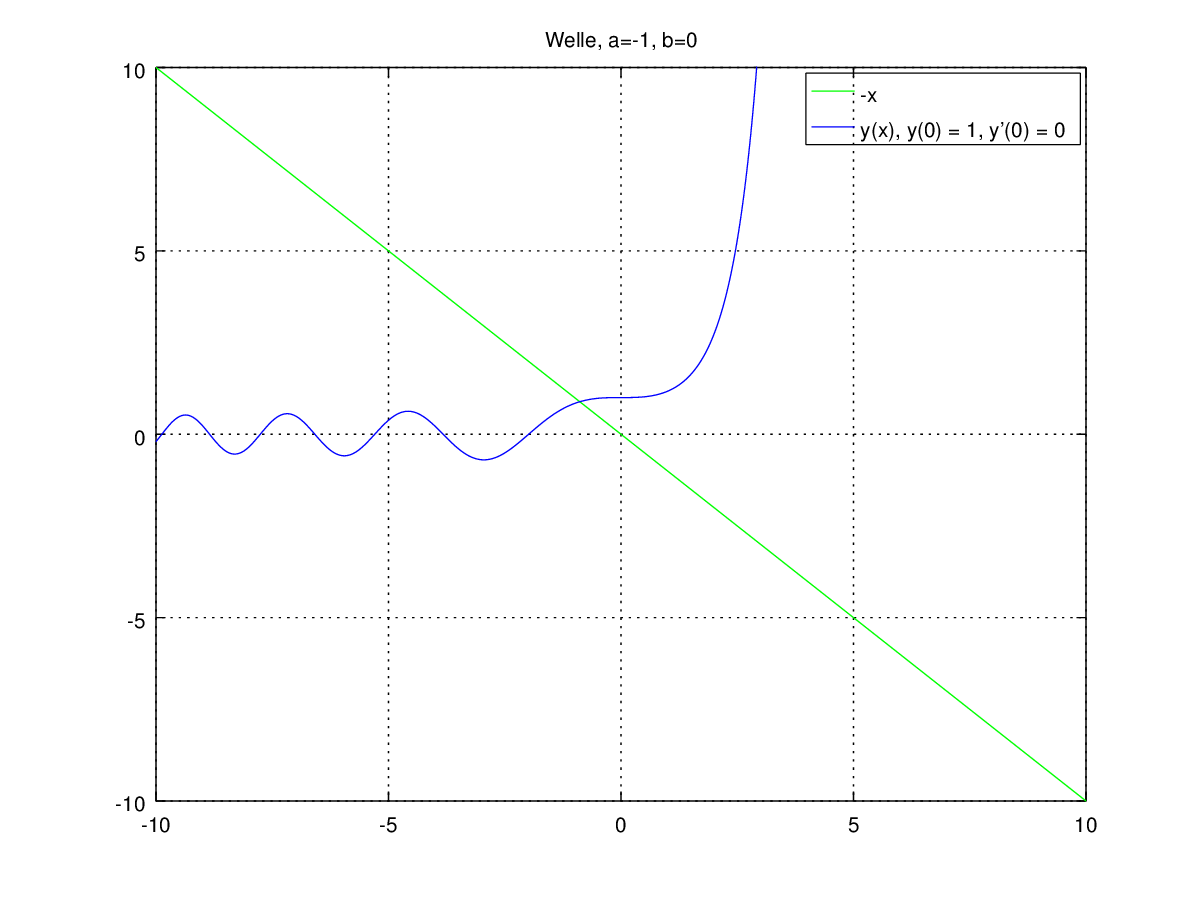
\includegraphics[scale=0.53]{./wellen/images/allgemein/n1.png}
\end{center}

\subsection{Beispiel: $n = 4$}

Auch ein Polynom 4-ten Grades stellt kein Problem dar. Die 
Differentialgleichung:

\begin{equation*}
	y''+(ax^4+bx^3+cx^2+dx+e)y = 0
\end{equation*}
ergibt nach dem Einsetzen:

\begin{align*}
	y(x) &= a_0+a_1x-\sum_{k=2}^{\infty} \frac{1}{k(k-1)} (aa_{k-2-4} + 
	ba_{k-2-3} + ca_{k-2-2} + da_{k-2-1} +ea_{k-2-0})x^k
	\\
	&= a_0+a_1x-\sum_{k=2}^{\infty} \frac{1}{k(k-1)} (aa_{k-6} + ba_{k-5} + 
	ca_{k-4} + da_{k-3} +ea_{k-2})x^k, \qquad a_{k<0} = 0
\end{align*}

Auch hier kann man graphisch die "Uberg"ange zwischen $\sin$ und $\cos$ bei 
positiven und $\sinh$ und $\cosh$ bei negativen Polynoml"osungen klar erkennen.

\begin{center}
	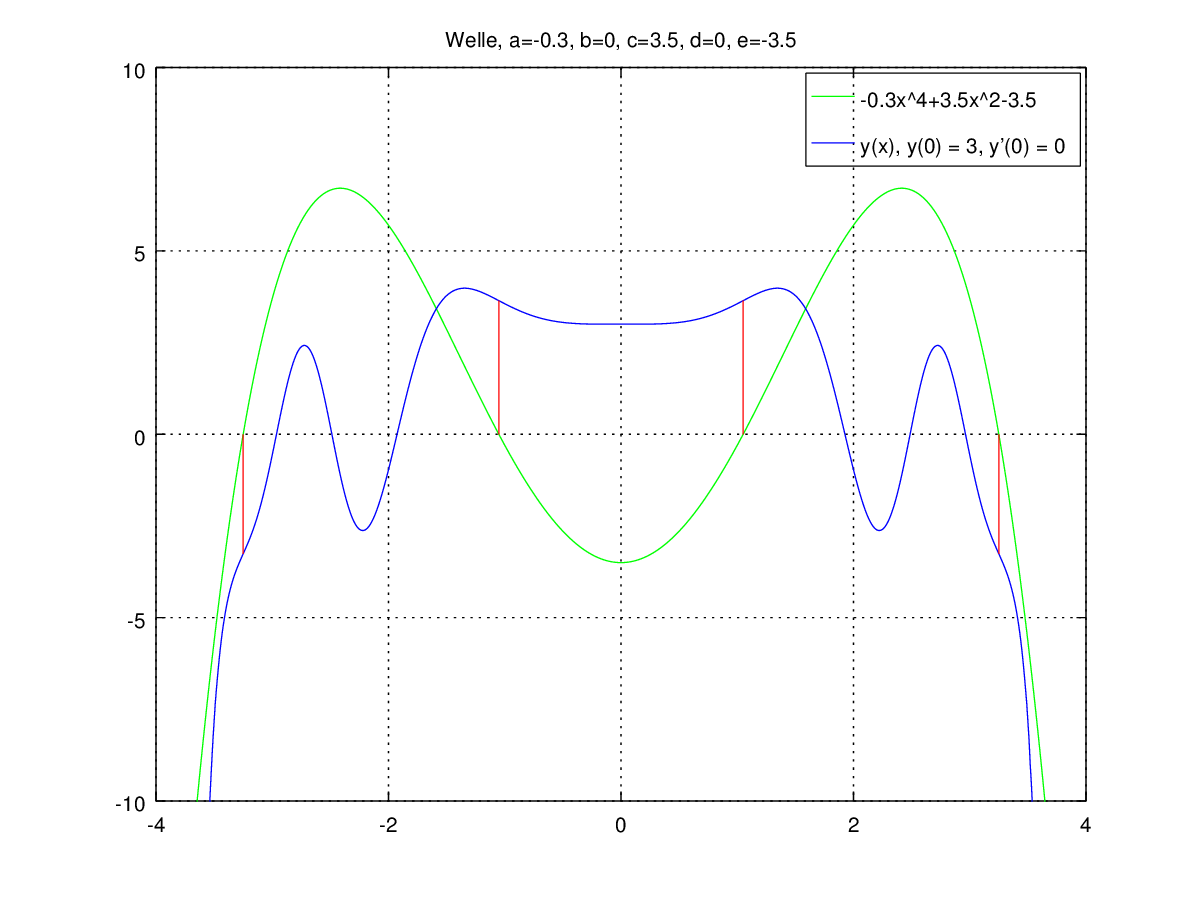
\includegraphics[scale=0.55]{./wellen/images/allgemein/n4.png}
\end{center}